\documentclass{article}
\usepackage{tikz}
\usepackage{pgfplots}
\usepackage{xcolor}

% 定义颜色
\definecolor{upurple}{RGB}{155,89,182}
\definecolor{udark}{RGB}{77,153,77}
\definecolor{ublue}{RGB}{52,152,219}
\definecolor{ured}{RGB}{231,76,60}
\definecolor{ugreen}{RGB}{46,204,113}


% 导入必要的库
\usepackage{amssymb}
\usetikzlibrary{shapes.geometric}
\usetikzlibrary{arrows,decorations.pathmorphing,backgrounds,positioning,fit,petri}
\usetikzlibrary{arrows.meta,fit,shapes.arrows}
\usepackage{caption}
\usepackage{subfig}
\usetikzlibrary{positioning,shapes,arrows,shadows,patterns}
\usetikzlibrary{calc}

% 设置pgfplots参数
\pgfplotsset{
    width=0.8\textwidth, % 图表宽度
    height=0.3\textheight, % 图表高度
    grid=major, % 显示主网格
    major grid style={dotted}, % 主网格样式
    symbolic x coords={WMT22,IWSLT17,AVG}, % x轴标签
    legend style={
        at={(0.5,0.95)}, % 图例位置
        anchor=north, % 图例锚点
        legend columns=2 % 图例列数
    },
}

% 设置图例与下文的间距
\captionsetup{belowskip=-10pt}

\begin{document}
\begin{figure}[t]
  \centering
  
  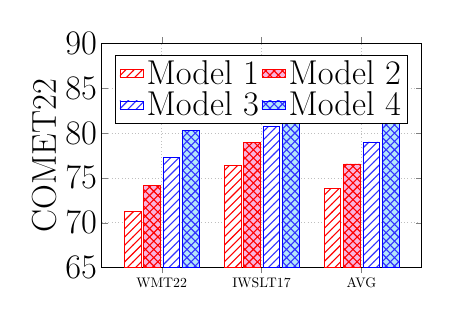
\begin{tikzpicture}[scale=0.5]
    \begin{axis}[
        ybar, % 使用柱状图
        bar width=1.2em, % 柱状图宽度
        enlarge x limits=0.3, % 增加x轴限度
        ylabel={\Huge{COMET22}}, % y轴标签
        xtick=data, % 使用数据点作为x轴标签
        ymin=65, ymax=90, % y轴范围
        ytick={60,65,70,75,80,85,90}, % y轴刻度位置
        yticklabels={\Huge{60},\Huge{65},\Huge{70},\Huge{75},\Huge{80},\Huge{85},\Huge{90}}, % y轴刻度标签
        width=0.8\textwidth, % 轴宽度
        height=0.6\textwidth, % 轴高度
        ylabel style={yshift=0pt,}, % y轴标签样式
        xticklabel style={yshift=0pt, } % x轴标签样式
    ]
    % 绘制柱状图，每个模型对应一个颜色
   \addplot+ [fill=white,draw=red, area legend,postaction={pattern=north 
east lines},pattern color=red] coordinates {(WMT22,71.26040225) (IWSLT17,76.42141589) (AVG,73.84090907)};
    \addplot+ [fill=magenta!30,draw=red, area legend,postaction={pattern=crosshatch},pattern color=red] coordinates {(WMT22,74.20203974) (IWSLT17,78.92049729) (AVG,76.56126851	)};
    \addplot+ [fill=white, draw=blue, area legend,postaction={pattern=north 
east lines},pattern color=blue!80] coordinates {(WMT22,77.29298931) (IWSLT17,80.7341152) (AVG,79.01355226)};
    \addplot+ [fill=cyan!30, draw=blue, area legend,postaction={pattern=crosshatch },pattern color=blue!80] coordinates {(WMT22,80.26201353) (IWSLT17,83.04977006) (AVG,81.6558918)};
    % 图例
    \legend{\Huge{Model 1}, \Huge{Model 2},  \Huge{Model 3},  \Huge{Model 4}}
    \end{axis}
  \end{tikzpicture}
  \caption{Comparison of COMET22 scores for different models on WMT22 and IWSLT2017 datasets} % 图标题
  \label{fig:mono-translate} % 图标签
\end{figure}
\end{document}
